%
%===============>>  ГРУППА 8-1 МОДУЛЬ 7  <<=============
%
\setmodule{7}

%BEGIN_FOLD % ====>>_____ Занятие 1 _____<<====
\begin{class}[number=1]
	\begin{listofex}
		\item Занятие 1
	\end{listofex}
\end{class}
%END_FOLD

%BEGIN_FOLD % ====>>_____ Занятие 2 _____<<====
\begin{class}[number=2]
	\begin{listofex}
		\item В прямоугольном треугольнике два катета равны \( 3 \) и \(  4 \). Найдите гипотенузу.
		\item Катеты прямоугольного треугольника равны \( 5 \) и \( 12 \). Чему равна гипотенуза?
		\item В прямоугольном треугольнике гипотенуза равна \( 20 \), а один из катетов равен \( 12 \). Чему равен другой катет?
		\item В прямоугольном треугольнике один из катетов равен \( 8 \), гипотенуза этого треугольника равна \( 17 \). Чему равен второй катет?
		\item Катет прямоугольного треугольника равен \( 7 \), а гипотенуза равна \( 25 \). Найдите длину второго катета.
		\item В равнобедренном прямоугольном треугольнике гипотенуза равна  \( 14\sqrt{2} \). Найдите длину катетов.
		\item Основание равнобедренного треугольника равно \( 16 \), боковая сторона равна \( 10 \). Чему равна высота проведенная к основанию этого треугольника?
		\item Боковая сторона равнобедренного треугольника равна \( 13 \), а длина основания равна \( 10 \). Найдите площадь этого треугольника.
		\item Найдите высоты равностороннего треугольника, если известно, что его сторона равна \( 8\sqrt{2} \).
		\item Дан параллелограмм \( ABCD \), где \( AB=15 \), \( AD=9 \). Также известно, что высота из точки \( B \) к основанию \( AD \) падает на точку \( D \). Чему равна площадь параллелограмма?
		\item Диагонали ромба равны \( 12 \) и \( 16 \) см. Чему равен периметр? Чему равна площадь? 
		\item Найдите все углы параллелограмма, если сумма двух из них равна \( 100^{\circ}\).
		\item В параллелограмме биссектриса угла \( А \) делит сторону \( ВС  \) на отрезки, равные \( 3 \) и \( 5  \) см. Найдите его периметр.
		\item Найдите углы параллелограмма, зная, что один из них больше другого на \( 50^{\circ} \).
	\end{listofex}
\end{class}
%END_FOLD

<<<<<<< HEAD
%BEGIN_FOLD % ====>>_____ Занятие 2 _____<<====
\begin{class}[number=2]
	\begin{listofex}
		\item Миша прошел от дома по направлению на восток \( 800 \) м. Затем повернул на север и прошел \( 600 \) м. На каком расстоянии (в метрах) от дома оказался Миша?
		\item Полина прошла от дома по направлению на запад \( 500 \) м. Затем повернула на север и прошла \( 300 \) м. После этого она повернула на восток и прошла еще \( 100 \) м. На каком расстоянии (в метрах) от дома оказалась Полина?
		\item Точка крепления троса, удерживающего флагшток в вертикальном положении, находится на высоте \( 15 \) м от земли. Расстояние от основания флагштока до места крепления троса на земле равно \( 8 \) м. Найдите длину троса.
		\item Пожарную лестницу длиной \( 13 \) м приставили к окну пятого этажа дома. Нижний конец лестницы отстоит от стены на \( 5 \) м. На какой высоте расположено окно? Ответ дайте в метрах.
		\item Высота равнобедренного треугольника равна \( 20 \) см, а его основание --- \( 10 \) см. Найдите его боковую сторону.
		\item Найдите площадь и периметр прямоугольника, сторона которого равна \( 9 \) см, а диагональ --- \( 15 \) см.
		\item Дан параллелограмм \( ABCD \), где \( AB=15 \), \( AD=9 \). Также известно, что высота из точки \( B \) к основанию \( AD \) падает на точку \( D \). Чему равна площадь параллелограмма?
		\item Диагонали ромба равны \( 12 \) и \( 16 \) см. Чему равен периметр? Чему равна площадь? 
		\item Найдите все углы параллелограмма, если сумма двух из них равна \( 100^{\circ}\).
		\item В параллелограмме биссектриса угла \( А \) делит сторону \( ВС  \) на отрезки, равные \( 3 \) и \( 5  \) см. Найдите его периметр.
		\item Найдите углы параллелограмма, зная, что один из них больше другого на \( 50^{\circ} \).
	\end{listofex}
\end{class}
%END_FOLD

=======
>>>>>>> 8fed5cac0b315f46d8969aae6889472e481d6473
%BEGIN_FOLD % ====>>_ Домашняя работа 1 _<<====
\begin{homework}[number=1]
	\begin{listofex}
		\item Стороны прямоугольника имеют длину \( 8 \) и \( 15 \) см. Найдите длину его диагонали.
		\item Пожарную лестницу приставили к окну, расположенному на высоте \( 12 \) м от земли. Нижний конец лестницы отстоит от стены на \( 5 \) м. Какова длина лестницы? Ответ дайте в метрах.
		\item Точка крепления троса, удерживающего флагшток в вертикальном положении, находится на высоте \( 6,3 \) м от земли. Расстояние от основания флагштока до места крепления троса на земле равно \( 1,6 \) м. Найдите длину троса в метрах.
		\item Один из острых углов прямоугольного треугольника составляет \( 30\degree \), а его гипотенуза равна \( 10 \). Найдите оба катета.
		\item Решите квадратное уравнение:
		\[x(x-5)=1-4x\]
	\end{listofex}
\end{homework}
%END_FOLD

%BEGIN_FOLD % ====>>_____ Занятие 3 _____<<====
\begin{class}[number=3]\begin{definit}
		\textbf{Синусом} острого угла прямоугольного треугольника называется отношение противолежащего катета к гипотенузе.
	\end{definit}
	\begin{definit}
		\textbf{Косинусом} острого угла прямоугольного треугольника называется отношение прилежащего катета к гипотенузе.
	\end{definit}
	\begin{listofex}
		\item В треугольнике \( ABC \) угол \( C \) равен \( 90 \) градусов, \( AC=6 \), \( AB=20 \). Найдите \( \sin B \).
		\item  В треугольнике \( ABC \) угол \( C \) равен \( 90 \) градусов, \( BC=9 \), \( AB=20 \). Найдите \( \cos B \).
		\item Найдите синус, косинус углов \( A \) и \( B \) треугольника \( ABC \) с прямым углом \( C \), если:
		\begin{tasks}(2)
			\task \( BC=8 \), \( AB=17 \)
			\task \( BC=21 \), \( AC=20 \)
			\task \( BC=1 \), \( AC=2 \)
		\end{tasks}
		
		\item В треугольнике \( ABC \) угол \( C \) прямой, \( BC=8 \), \( \sin A=0,4 \). Найдите \( AB \).
		\item В треугольнике \( ABC \) угол \( C \) прямой, \( AC=15 \), \( \cos A=\dfrac{5}{7} \). Найдите \( AB \).
		\item В треугольнике \( ABC \) угол \( C \) равен \( 90\degree \), \( BC=12 \), \( \sin A=\dfrac{4}{11} \). Найдите \( AB \).
		\item Катеты прямоугольного треугольника равны \( \sqrt{15} \) и \( 1 \). Найдите синус наименьшего угла этого треугольника.
		\item В треугольнике \( ABC \) угол \( C \) равен \( 90\degree \), \( \sin A=\dfrac{4}{5} \), \( AC=9 \). Найдите \( AB \).
		\item  Есть прямоугольный треугольник \( ABC \), где \( \angle C=90^{\circ} \), и \( AC=7 \), \( AB=25 \). Найдите длину \( BC \).
		\item Сумма двух углов параллелограмма равна \( 62^{\circ} \). Найдите один из оставшихся углов. Ответ дайте в градусах.
		\item Две стороны параллелограмма относятся как \( 9:11 \), а периметр его равен \( 40 \). Найдите большую сторону параллелограмма.
	\end{listofex}
\end{class}
%END_FOLD

%BEGIN_FOLD % ====>>_____ Занятие 4 _____<<====
\begin{class}[number=4]
	\begin{listofex}
		\item 
		\begin{minipage}[t]{\bodywidth}
		Найдите синус и косинус угла AOB, изображенного на рисунке.
	\end{minipage}
	\hspace{0.02\linewidth}
	\begin{minipage}[t]{\picwidth}
		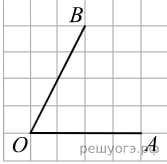
\includegraphics[align=t, width=\linewidth]{\picpath/G81M7L4-1}
	\end{minipage}
	\item Найдите синус, косинус углов \( A \) и \( B \) треугольника \( ABC \) с прямым углом \( C \), если:
	\begin{tasks}(2)
		\task \( BC=4 \), \( AB=12 \)
		\task \( BC=3 \), \( AC=5 \)
		\task \( BC=13 \), \( AC=24 \)
	\end{tasks}
	\end{listofex}
		\begin{definit}
			\textbf{Основное тригонометрическое тождество }
			\begin{tasks}(3)
				\task[]
				\task[] \( \sin ^{2} x+\cos ^{2} x=1  \)
				\task[]
			\end{tasks} 
		\end{definit}
		\begin{listofex}[resume]
		\item Найдите:
		\begin{tasks}(2)
			\task \( \sin\alpha \), если \( \cos\alpha=\dfrac{1}{2} \)
			\task \( \cos\alpha \), если \( \sin\alpha=\dfrac{\sqrt{3}}{2} \)
		\end{tasks}
		\item Вычислить \( \sin \alpha \), если \( \cos \alpha =\dfrac{3}{5}^{\circ} \)	и \( 0 < \angle < \dfrac{\pi}{2} \).
		\item В треугольнике \( ABC  \) угол \( C \) равен \( 90^{\circ} \), \( \sin B = \dfrac{4}{15} \) , \( AB=45 \). Найдите \( AC \).
		\item В треугольнике \( ABC \) угол \( C \) прямой, \( AC=18 \), \( \cos A=\dfrac{6}{13} \). Найдите \( AB \).
		\item В треугольнике \( ABC \) угол \( C \) равен \( 90^{\circ} \), \( AC  =  4 \),  \(  \cos A = 0,5 \). Найдите \( AB \).  
		\item Катеты прямоугольного треугольника равны \( 4\sqrt{6} \) и 2. Найдите синус наименьшего угла этого треугольника.
		\item Найдите синус и косинус  большего острого угла прямоугольного треугольника с катетами \( 7 \) см и \( 24  \) см.
		\item Периметр равнобедренного треугольника равен \( 64 \) см, косинус угла при основании равен \( 0,6 \). Найдите площадь треугольника.
		\item В равнобедренном треугольнике \( ABC \) с основанием \( AB \) боковая сторона равна \( 16\sqrt{15} \),  \( \sin\angle BAC=0,25 \). Найдите длину высоты \( AH \).
		\item Площадь параллелограмма равна \( 40 \), а две его стороны равны \( 5  \) и \( 10 \). Найдите его высоты.
	\end{listofex}
\end{class}
%END_FOLD

%BEGIN_FOLD % ====>>_ Домашняя работа 2 _<<====
\begin{homework}[number=2]
	\begin{listofex}
		\item В треугольнике \( ABC \) угол \( C \) прямой, \( BC=12 \), \( \sin A=\dfrac{6}{13} \). Найдите \( AB \).
		\item В треугольнике \( ABC \) угол \( C \) прямой, \( BC=15 \), \( \cos B=\dfrac{18}{30} \). Найдите \( AB \).
		\item  Высота треугольника равна \( 10 \) и образует с прилежащими сторонами углы \( 45\degree \) и \( 60\degree \). Найдите стороны треугольника.
		\item  В параллелограмме \( ABCD \) \( CH \) --- высота, \( AB = 4 \), \( \cos C = 0,8 \). Найдите \( CH \).
		\item  В треугольнике \( ABC \) \( AB = BC = 10 \), \( \sin A = 0,2 \). Найдите \( AC \).
		\item Вычислите \( \cos \alpha \), если \( \sin \alpha =\dfrac{12}{13} \). Угол \( \alpha \) острый.
		\item Катеты прямоугольного треугольника равны \( \sqrt{19} \) и \( 9 \). Найдите синус наименьшего угла этого треугольника.
	\end{listofex}
\end{homework}
%END_FOLD

%BEGIN_FOLD % ====>>_____ Занятие 5 _____<<====
\begin{class}[number=5]
	\begin{listofex}
		\item Занятие 5
	\end{listofex}
\end{class}
%END_FOLD

%BEGIN_FOLD % ====>>_____ Занятие 6 _____<<====
\begin{class}[number=6]
	\begin{listofex}
		\item Занятие 6
	\end{listofex}
\end{class}
%END_FOLD

%BEGIN_FOLD % ====>>_ Домашняя работа 3 _<<====
\begin{homework}[number=3]
	\begin{listofex}
		\item Домашняя работа 3
	\end{listofex}
\end{homework}
%END_FOLD

%BEGIN_FOLD % ====>>_____ Занятие 7 _____<<====
\begin{class}[number=7]
	\title{Подготовка к проверочной}
	\begin{listofex}
		\item Занятие 7
	\end{listofex}
\end{class}
%END_FOLD

=%BEGIN_FOLD % ====>>_ Проверочная работа _<<====
\begin{exam}
	\begin{listofex}
		\item Проверочная
	\end{listofex}
\end{exam}
%END_FOLD

%BEGIN_FOLD % ====>>_ Консультация _<<====
\begin{consultation}
	\begin{listofex}
		\item Постройте график \( y=|x| \) и определите: 
		\begin{tasks}(1)
			\task Промежутки возрастания функции;
			\task Промежутки убывания функции;
			\task Область определения функции;
			\task Область значений функции.
		\end{tasks}
		\item Постройте график \( y=-|x| \) и определите: 
		\begin{tasks}(1)
			\task Промежутки возрастания функции;
			\task Промежутки убывания функции;
			\task Область определения функции;
			\task Область значений функции.
		\end{tasks}
		\item Постройте график \( y=|x|-3 \)
	\end{listofex}
	\newpage
	\title{Домашняя работа}
	\begin{listofex}
		\item Постройте график \( y=|x|+1 \)
	\end{listofex}
\end{consultation}
%END_FOLD